\documentclass[a4paper,10pt]{article}

% Encoding and typeface: XeLaTeX with Latin Modern Roman (fontspec default), English via polyglossia
\usepackage{fontspec}
\usepackage{polyglossia}
\setdefaultlanguage[variant=british]{english}

% Layout (tight margins)
\usepackage[a4paper,top=1.2cm,bottom=1.3cm,left=1.3cm,right=1.3cm]{geometry}

% Typography
\usepackage{microtype}
\usepackage{setspace}
\setstretch{0.92}

% Paragraph settings
\setlength{\parindent}{0pt}
\setlength{\parskip}{3pt}

% Section styling
\usepackage{titlesec}
\titleformat{\section}{\bfseries\normalsize}{\thesection.}{0.4em}{}
\titlespacing*{\section}{0pt}{6pt}{3pt}

% Better lists
\usepackage{enumitem}
\setlist{noitemsep, topsep=2pt}

% Mathematics, tables, figures
\usepackage{amsmath}
\usepackage{booktabs}
\usepackage{graphicx}
\usepackage[font=small,labelfont=bf,labelsep=period,skip=3pt]{caption}
\setlength{\textfloatsep}{8pt}
\setlength{\floatsep}{6pt}

\newcommand{\VoneCreditL}{-0.76}
\newcommand{\VoneCreditLp}{0.969}
\newcommand{\VoneCreditD}{2.42}
\newcommand{\VoneCreditDp}{1.000}
\newcommand{\VoneCreditDD}{-4.16}
\newcommand{\VoneCreditDDp}{0.005}
\newcommand{\VoneUsdL}{-2.35}
\newcommand{\VoneUsdLp}{0.407}
\newcommand{\VoneUsdD}{-12.06}
\newcommand{\VoneUsdDp}{$<$0.001}
\newcommand{\VoneTufeL}{2.55}
\newcommand{\VoneTufeLp}{1.000}
\newcommand{\VoneTufeD}{-1.38}
\newcommand{\VoneTufeDp}{0.868}
\newcommand{\VoneTufeDD}{-4.99}
\newcommand{\VoneTufeDDp}{$<$0.001}
\newcommand{\Months}{127}
\newcommand{\TufeRatio}{10.7}
\newcommand{\CreditRatio}{38}
\newcommand{\ItoRatio}{13.8}
\newcommand{\FiveFridays}{44}
\newcommand{\FriCoef}{0.229}
\newcommand{\FriSe}{0.008}
\newcommand{\LogFiveFour}{0.223}
\newcommand{\FriRsq}{0.87}
\newcommand{\NextRsq}{0.31}
\newcommand{\DtufeFirst}{1.5}
\newcommand{\DtufeLast}{69.6}
\newcommand{\InflFirst}{0.61}
\newcommand{\InflLast}{3.34}
\newcommand{\TufeDcAICp}{0.137}
\newcommand{\TufeDcAICk}{6}
\newcommand{\TufeDcBICp}{$<$0.001}
\newcommand{\TufeDcBICk}{0}
\newcommand{\TufeDctAICp}{0.014}
\newcommand{\TufeDkpss}{1.24}
\newcommand{\ItoDcAICp}{0.112}
\newcommand{\ItoDcAICk}{2}
\newcommand{\ItoDkpss}{1.31}
\newcommand{\KpssCv}{0.463}
\newcommand{\RealDcAICp}{0.269}
\newcommand{\RealDcAICk}{12}
\newcommand{\RealDcBICp}{$<$0.001}
\newcommand{\RealDcBICk}{0}
\newcommand{\RealDkpssp}{0.088}
\newcommand{\RealAcfTwelve}{0.39}
\newcommand{\NomDcAICp}{0.793}
\newcommand{\UsdLcp}{0.735}
\newcommand{\UsdLctp}{0.407}
\newcommand{\UsdDcp}{$<$0.001}
\newcommand{\ZaTufe}{-6.16}
\newcommand{\ZaTufeBreak}{2021-10}
\newcommand{\ZaTufeBefore}{0.99}
\newcommand{\ZaTufeAfter}{4.18}
\newcommand{\ZaIto}{-5.69}
\newcommand{\ZaItoBreak}{2021-09}
\newcommand{\ZaItoBefore}{0.98}
\newcommand{\ZaItoAfter}{4.84}
\newcommand{\ZaCvOne}{-5.28}
\newcommand{\ZaCvFive}{-4.81}
\newcommand{\ZaUsdL}{-4.32}
\newcommand{\ZaUsdD}{-12.62}
\newcommand{\ZaReal}{-4.41}
\newcommand{\ZaRealLags}{12}
\newcommand{\ZaTufeLags}{6}
\newcommand{\ZaTufeTheta}{2.97}
\newcommand{\ZaTufeTtheta}{4.53}
\newcommand{\ZaTufeTbeta}{1.16}
\newcommand{\ZaItoTheta}{2.61}
\newcommand{\ZaItoTtheta}{4.10}
\newcommand{\ZaItoTbeta}{0.41}
\newcommand{\OrderRealAIC}{2}
\newcommand{\OrderRealBIC}{1}
\newcommand{\OrderUsdAIC}{1}
\newcommand{\OrderUsdBIC}{1}
\newcommand{\OrderTufeAIC}{2}
\newcommand{\OrderTufeBIC}{1}
\newcommand{\OrderItoAIC}{2}
\newcommand{\OrderItoBIC}{2}
\newcommand{\OrderNomAIC}{2}
\newcommand{\OrderNomBIC}{1}


\begin{document}

% Header (top-right)
\begin{flushright}
\small \textbf{Compiled on:} \today
\end{flushright}

\vspace{-6pt}
\hrule
\vspace{24pt}

\textbf{TITLE:} Unit roots in four Turkish monthly series: what the ADF test says once the data, the model and the lags are examined

\textbf{SUBJECT:} Aim, method and results of the analyses in version 2 of the \texttt{ADF\_Unit\_Root} repository

\textbf{PREPARED BY:} Muhammed İkbal Yılmaz (myucanlar@gmail.com)

\vspace{12pt}

\section{Aim and scope}

Version 1 of this project determined the order of integration of three monthly series from March 2014 to September 2024
(\Months{} months): bank and credit card spending (\texttt{credit}, thousand TRY), the weighted average interest rate on USD
commercial loans (\texttt{usd}, percent) and the consumer price index (\texttt{tufe}, 2003 = 100). It used the augmented
Dickey--Fuller (ADF) test on the series in levels, with a constant and a trend (Model 3), at most 14 lagged differences chosen by
AIC, and tested upward from the level. It found \texttt{credit} and \texttt{tufe} to be $I(2)$ and \texttt{usd} to be $I(1)$.
Version 2 keeps the test, the three models of version 1 and its lag settings, and adds the fourth series of the data file, a price
index of the Istanbul Chamber of Commerce (\texttt{ito}), as an independent check on the CPI. It asks three questions:

\begin{enumerate}
  \item \textbf{What do the series contain before they are tested?} Calendar effects and exponential growth change what a unit
  root test in levels measures.
  \item \textbf{Does the order of integration depend on the ADF model and on the lag criterion?} Version 1 defined three models but
  used only one, and one criterion.
  \item \textbf{Is inflation non-stationary, or stationary around a structural break?} Version 1 named break tests as the next
  step but did not run them.
\end{enumerate}

\section{Data and notation}

Let $C_t$ be card spending, $R_t$ the USD loan rate, $P_t$ the CPI and $Q_t$ the ITO index in month $t = 1, \dots, \Months$, and
$F_t \in \{4, 5\}$ the number of Fridays in month $t$. Version 2 analyses
\begin{align}
c_t &= \log (C_t / F_t), & c^{r}_t &= \log \bigl(C_t / (F_t P_t)\bigr), & p_t &= \log P_t, & q_t &= \log Q_t, & R_t, \label{eq:series}
\end{align}
that is, log card spending per week, log real card spending per week, log prices and the loan rate as published. Monthly inflation
is $\pi_t = 100\,\Delta p_t$, where $\Delta y_t = y_t - y_{t-1}$ and $\Delta^d = \Delta(\Delta^{d-1})$.

\textbf{Why per week.} If the monthly figure is the sum of the weekly figures $W_w$ of the weeks ending on a Friday in month $t$,
then $C_t = F_t \bar W_t$, with $\bar W_t$ the average week, and
\begin{equation}
\Delta \log C_t = \Delta \log \bar W_t + \Delta \log F_t, \qquad \Delta \log F_t \in \{0, \pm\log(5/4)\} = \{0, \pm \LogFiveFour\}.
\label{eq:calendar}
\end{equation}
Analysis 1 estimates $\Delta \log C_t = a + b\,\Delta F_t + u_t$ by OLS for $F_t$ and for the count of each other weekday; under
\eqref{eq:calendar}, $b \approx \log(5/4)$ for Fridays. Dividing by $F_t$ removes this term.

\textbf{Why logs.} If $X_t = X_0 e^{g t}$, then $\Delta X_t = X_{t-1}(e^{g} - 1)$ grows with the level, while $\Delta \log X_t = g$ is
constant. A growth rate without trend therefore gives a first difference in levels with a trend, and a test in levels mixes the two.

\section{Models and tests}

\textbf{Order of integration.} A series is $I(d)$ if $\Delta^{d} y_t$ is stationary and $\Delta^{d-1} y_t$ is not. In
$y_t = \rho\, y_{t-1} + u_t$ with stationary $u_t$, $\rho = 1$ (a unit root) gives $I(1)$; $|\rho| < 1$ gives $I(0)$.

\textbf{ADF test} (Dickey and Fuller, 1979; Said and Dickey, 1984). For a series $y_t$ (a level or a difference) the regression is
\begin{equation}
\Delta y_t = \delta' \mathbf{d}_t + \gamma\, y_{t-1} + \sum_{j=1}^{k} \phi_j\, \Delta y_{t-j} + \varepsilon_t, \qquad
\gamma = \rho - 1, \label{eq:adf}
\end{equation}
with the deterministic terms of the three models of version 1: Model 1, $\mathbf{d}_t$ empty; Model 2, $\mathbf{d}_t = 1$; Model 3,
$\mathbf{d}_t = (1, t)'$. The lagged differences absorb the autocorrelation of $u_t$. The hypotheses are $H_0\colon \gamma = 0$ (unit
root) and $H_1\colon \gamma < 0$ (stationary, around zero, a constant or a linear trend in Models 1--3). The statistic is
$\tau = \hat\gamma / \operatorname{se}(\hat\gamma)$ from OLS. Under $H_0$ it does not follow a $t$ distribution; its distribution
depends on the model, and $p$-values come from MacKinnon's (1994) approximate distribution functions and critical values from
MacKinnon (2010), as implemented in \texttt{statsmodels}. The test rejects for $\tau$ below the critical value.

\textbf{Number of lags.} For each $k = 0, 1, \dots, 14$, regression \eqref{eq:adf} is estimated on the same $T^\ast = N - 1 - 14$
observations ($N$ the length of the series tested), so that the criteria are comparable, and $k$ minimises
\begin{equation}
\mathrm{AIC}(k) = -2\,\ell_k + 2\,m_k, \qquad \mathrm{BIC}(k) = -2\,\ell_k + m_k \log T^\ast, \label{eq:ic}
\end{equation}
where $\ell_k = -\tfrac{T^\ast}{2}\bigl(\log 2\pi + \log(\mathrm{SSR}_k / T^\ast) + 1\bigr)$ is the Gaussian log-likelihood of the
OLS fit and $m_k$ its number of coefficients. Regression \eqref{eq:adf} with the chosen $k$ is then re-estimated on all
$N - 1 - k$ usable observations, and $\tau$ is taken from that fit. AIC with $k \le 14$ is the setting of version 1; BIC, whose
penalty is larger ($\log T^\ast \approx 4.7$ against 2), is added for comparison. Figure~\ref{fig:lags} also shows $\tau$'s $p$-value
for every fixed $k$.

\textbf{Order of testing} (Dickey and Pantula, 1987). Each ADF test assumes at most one unit root in the series it is applied to.
The order is therefore found from the top down: test $\Delta^2 y_t$; if the unit root is rejected (5\% level), test $\Delta y_t$; if
rejected again, test $y_t$. The order is the number of differences of the last series in which the unit root was not rejected, plus
one; if every test rejects, the order is 0. Version 1 tested upward from the level, which violates the assumption when the series
has two unit roots.

\textbf{Model for each difference.} Levels of trending series ($c_t$, $c^r_t$, $p_t$, $q_t$) use Model 3: a random walk with drift,
$y_t = \mu + y_{t-1} + u_t$, has a linear trend, so the stationary alternative must allow one. $R_t$, an interest rate with no reason
to trend, uses Model 2. Differences use Model 2: $\Delta y_t = a + b\,t + \dots$ would mean a quadratic trend in $y_t$.

\textbf{KPSS test} (Kwiatkowski et al., 1992), with the hypotheses reversed. Write $y_t = \xi'\mathbf{d}_t + r_t + e_t$ with
$r_t = r_{t-1} + u_t$; $H_0\colon \operatorname{Var}(u_t) = 0$ (stationary around $\xi'\mathbf{d}_t$), $H_1$: a unit root. With
$\hat e_t$ the OLS residuals of $y_t$ on $\mathbf{d}_t$ ($\mathbf{d}_t = 1$, or $(1, t)'$ for levels of trending series),
$S_t = \sum_{s \le t} \hat e_s$ and $\hat\gamma_i = T^{-1}\sum_{t > i} \hat e_t \hat e_{t-i}$,
\begin{equation}
\eta = \frac{T^{-2} \sum_{t=1}^{T} S_t^2}{\hat\sigma^2_{\ell}}, \qquad
\hat\sigma^2_{\ell} = \hat\gamma_0 + 2 \sum_{i=1}^{\ell} \Bigl(1 - \frac{i}{\ell + 1}\Bigr) \hat\gamma_i, \label{eq:kpss}
\end{equation}
where $\hat\sigma^2_\ell$ is the Bartlett estimate of the long-run variance and $\ell$ is chosen by the automatic rule of
\texttt{statsmodels} (\texttt{nlags="auto"}). The test rejects for large $\eta$; the 5\% critical values are 0.463 (constant) and
0.146 (constant and trend). The $p$-value is interpolated in a table that ends at 0.01 and 0.10, so values outside are reported as
$\le 0.01$ or $\ge 0.10$.

\textbf{Zivot--Andrews test} (Zivot and Andrews, 1992), Model A, the \texttt{"c"} option of \texttt{statsmodels}. For a candidate
break $T_B$, with $DU_t = 1$ for $t > T_B$ and 0 otherwise,
\begin{equation}
\Delta y_t = \mu + \theta\, DU_t + \beta\, t + \alpha\, y_{t-1} + \sum_{j=1}^{k} c_j\, \Delta y_{t-j} + \varepsilon_t . \label{eq:za}
\end{equation}
$H_0\colon \alpha = 0$ (unit root); $H_1\colon \alpha < 0$, stationarity around a linear trend whose level shifts by $\theta/(-\alpha)$
after $T_B$. The statistic is the smallest $t_{\alpha}(T_B)$ over the candidate dates in the central 70\% of the sample (15\%
trimmed at each end), and the estimated break is the $T_B$ that attains it, i.e.\ the last month of the first regime. Because $T_B$ is chosen to favour
rejection, the critical values are more negative than those of the ADF test: $\ZaCvOne$ (1\%) and $\ZaCvFive$ (5\%), from a
simulated table. \texttt{statsmodels} chooses $k$ once, by AIC with $k \le 14$ in the ADF regression \eqref{eq:adf} with
$\mathbf{d}_t = (1, t)'$ and no break, and uses it for every $T_B$; the original paper chooses $k$ for each $T_B$ separately.

\textbf{From the equations to the code.} Every step is a function in \texttt{unitroots/} and is checked against an independent
computation in \texttt{tests/run\_tests.py}:

\begin{center}\footnotesize
\begin{tabular}{lll}
\toprule
Step & Equations & Code \\
\midrule
Series, Fridays & \eqref{eq:series}, \eqref{eq:calendar} & \texttt{load}, \texttt{fridays}, \texttt{transformed} (\texttt{data.py}) \\
ADF, lag choice & \eqref{eq:adf}, \eqref{eq:ic} & \texttt{adf(series, regression, maxlag=14, autolag)}; fixed $k$: \texttt{adf\_by\_lag} \\
Order of integration & top-down sequence & \texttt{integration\_order(series, \{0: "ct", 1: "c", 2: "c"\})} \\
KPSS & \eqref{eq:kpss} & \texttt{kpss\_test(series, regression)} \\
Zivot--Andrews & \eqref{eq:za} & \texttt{za\_test}; regression at the break: \texttt{za\_regression} \\
\bottomrule
\end{tabular}
\end{center}

\section{Analysis 1: What the series contain (Figure~\ref{fig:data})}

\textbf{Why.} A unit root test answers a question about the stochastic trend of a series. If part of the variation comes from the
calendar, or if the series grows exponentially, a test in levels also measures these properties.

\textbf{Method.} The ADF tests of version 1 are repeated with its settings: regression \eqref{eq:adf} on $C_t$, $R_t$ and $P_t$
in levels and differences, Model 3, $k \le 14$ by AIC. The calendar regression below \eqref{eq:calendar} is estimated for each
weekday. The CPI is shown as monthly changes in index points and as monthly changes
in its logarithm, i.e.\ monthly inflation.

\textbf{How to read the figure.} (a) Each point is a month; the horizontal axis is the change in the number of Fridays from the
previous month ($-1$, $0$ or $+1$, spread slightly for visibility). (b) and (c) show the same CPI changes in two units.

\begin{figure}[h]
\centering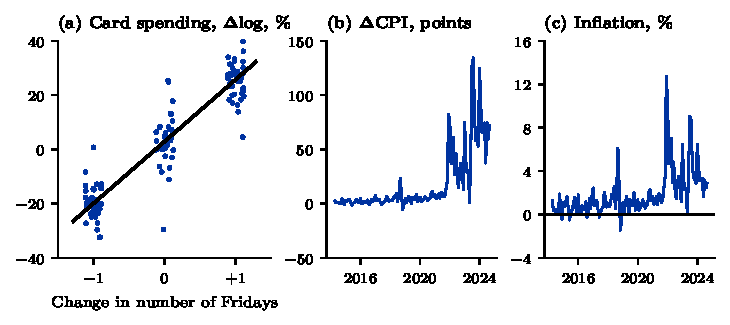
\includegraphics[width=\linewidth]{../figures/fig1_data.pdf}
\caption{(a) Monthly change in log card spending against the change in the number of Fridays in the month, with the OLS line.
(b) Monthly change in the CPI in index points. (c) Monthly inflation, $100\,\Delta\log$ CPI.}\label{fig:data}
\end{figure}

\textbf{Finding.} The ADF statistics of version 1 are reproduced exactly (for example $\VoneCreditL$, $\VoneCreditD$ and
$\VoneCreditDD$ for \texttt{credit} in level, first and second difference; $\VoneTufeL$, $\VoneTufeD$, $\VoneTufeDD$ for
\texttt{tufe}). The number of Fridays explains \FriRsq{} of the variance of the monthly change in log card spending (no other
weekday more than \NextRsq{}). One more Friday raises spending by \FriCoef{} in logs (standard error \FriSe{}), close to
$\log(5/4) = \LogFiveFour$, the change from summing four weekly values to summing five; \FiveFridays{} of the \Months{} months
have five Fridays. Over the sample the CPI rose by a factor of \TufeRatio{} and card spending by a factor of \CreditRatio{}. The
monthly change of the CPI in index points averaged \DtufeFirst{} in the first year and \DtufeLast{} in the last; monthly inflation
rose from \InflFirst\% to \InflLast\%.

\textbf{Interpretation.} The card spending data behave as sums of weekly figures for the weeks ending on a Friday; dividing by the
number of Fridays gives spending per week and removes this calendar component. For a series that grows exponentially, the change
in levels is roughly the level times the growth rate, so it trends upward even when the growth rate does not. A unit root found in
the first difference of the level is then partly a property of the level itself; in logs the first difference is the growth rate.
The $I(2)$ results of version 1 for \texttt{credit} and \texttt{tufe} were obtained in levels and therefore have to be re-examined
in logs.

\section{Analysis 2: Integration order, model and lags (Table~\ref{tab:grid}, Figure~\ref{fig:lags})}

\textbf{Why.} With 127 observations, the decision between a unit root and stationarity can depend on the deterministic terms and on
the number of lags; a reader should see whether it does.

\textbf{Method.} For $c^r_t$, $R_t$, $p_t$, $q_t$ in level and first difference: ADF $p$-values of \eqref{eq:adf} for
the three models with $k$ by AIC and for Model 2 with $k$ by BIC \eqref{eq:ic}, and the KPSS $p$-value of \eqref{eq:kpss}; then
the order of integration from the top down. Figure~\ref{fig:lags} shows the ADF $p$-value of the first differences (Model 2) for every number of
lags from 0 to 14.

\begin{table}[h]
\centering\footnotesize
\caption{ADF $p$-values (number of lags in parentheses) for Models 1--3 with AIC and Model 2 with BIC, and KPSS $p$-values
(trend-stationarity for levels of trending series, level-stationarity otherwise; reported within $[0.01, 0.10]$).}\label{tab:grid}
\begin{tabular}{lrrrrr}
\toprule
 & Model 1, AIC & Model 2, AIC & Model 3, AIC & Model 2, BIC & KPSS \\
\midrule
log real card spending per week & 0.959 (13) & 0.994 (13) & 0.971 (13) & 0.949 (0) & $\le$0.01 \\
$\Delta$ log real card spending per week & 0.123 (12) & 0.269 (12) & 0.176 (12) & $<$0.001 (0) & 0.088 \\
USD loan rate & 0.771 (0) & 0.735 (0) & 0.407 (14) & 0.735 (0) & $\le$0.01 \\
$\Delta$ USD loan rate & $<$0.001 (0) & $<$0.001 (0) & $<$0.001 (0) & $<$0.001 (0) & $\ge$0.10 \\
log CPI & 0.996 (7) & 0.999 (7) & 0.995 (7) & 1.000 (1) & $\le$0.01 \\
$\Delta$ log CPI & 0.225 (5) & 0.137 (6) & 0.014 (6) & $<$0.001 (0) & $\le$0.01 \\
log ITO index & 0.993 (3) & 0.999 (3) & 0.992 (3) & 0.999 (3) & $\le$0.01 \\
$\Delta$ log ITO index & 0.649 (13) & 0.112 (2) & 0.021 (2) & 0.112 (2) & $\le$0.01 \\
\bottomrule

\end{tabular}
\end{table}

\begin{figure}[h]
\centering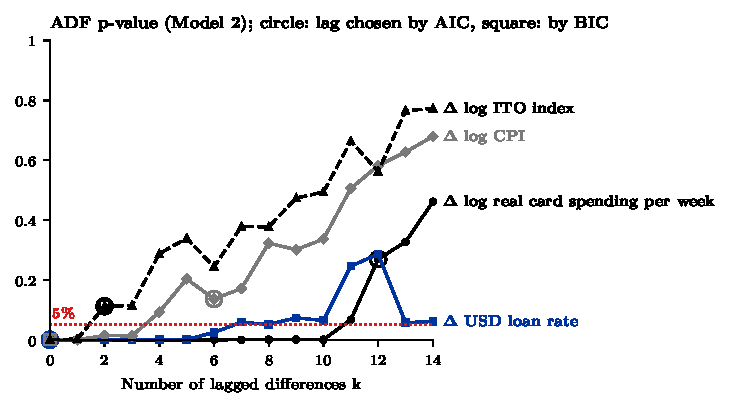
\includegraphics[width=0.92\linewidth]{../figures/fig2_lags.pdf}
\caption{ADF $p$-value (Model 2) of the first differences against the number of lagged differences. Circles and squares mark the
numbers of lags chosen by AIC and BIC. Dotted: 5\%.}\label{fig:lags}
\end{figure}

\textbf{How to read the figure.} A curve below the dotted line means that, with that many lags, the test rejects a unit root in the
differenced series. Where a curve crosses the line, the conclusion depends on the number of lags.

\textbf{Finding.} No level is found stationary: ADF rejects a unit root in no level, and KPSS rejects stationarity in every level. For the USD loan rate the first difference rejects a unit root for every
model, both criteria and every number of lags up to six (Model 2, AIC: $p$ \UsdDcp), and KPSS does not reject its stationarity:
\texttt{usd} is $I(1)$, as in version 1. For monthly inflation the result depends on the choices: for the CPI, Model 2 with AIC
(\TufeDcAICk{} lags) gives $p = \TufeDcAICp$, Model 3 gives $p = \TufeDctAICp$, and Model 2 with BIC (\TufeDcBICk{} lags) gives $p$
\TufeDcBICp; for the ITO index Model 2 gives $p = \ItoDcAICp$. KPSS rejects the stationarity of both inflation series (statistics
\TufeDkpss{} and \ItoDkpss{} against a 5\% critical value of \KpssCv). For real card spending per week, AIC keeps \RealDcAICk{} lags
and gives $p = \RealDcAICp$; BIC keeps \RealDcBICk{} and gives $p$ \RealDcBICp, and KPSS does not reject at 5\% ($p = \RealDkpssp$).
The autocorrelation of its growth at lag 12 is \RealAcfTwelve. Testing from the top down with AIC gives orders \OrderRealAIC{}
(real card spending), \OrderUsdAIC{} (\texttt{usd}), \OrderTufeAIC{} (CPI) and \OrderItoAIC{} (ITO); with BIC \OrderRealBIC,
\OrderUsdBIC, \OrderTufeBIC{} and \OrderItoBIC.

\textbf{Interpretation.} \texttt{usd} is clearly $I(1)$. For real card spending the AIC choice of 12 lags follows the annual
pattern of monthly spending (the lag-12 autocorrelation); with these lags the test loses power, while the other evidence points to
$I(1)$. For the price indices the ADF test alone does not settle between $I(1)$ and $I(2)$, and KPSS rejects a constant mean of
inflation. Both outcomes are also what a stationary series with a shift in its mean produces, which analysis 3 examines.

\section{Analysis 3: A break in inflation (Figure~\ref{fig:breaks})}

\textbf{Why.} A one-time shift in the mean of a stationary series makes the ADF test favour a unit root and the KPSS test reject
stationarity; this is the motivation of the Zivot--Andrews test. The question is whether monthly inflation is better
described as $I(1)$, or as stationary around a shift.

\textbf{Method.} Zivot--Andrews regression \eqref{eq:za} for $\Delta p_t$ and $\Delta q_t$ (monthly inflation of the two price
indices), and for comparison for $R_t$, $\Delta R_t$ and $\Delta c^r_t$. At the estimated break, regression \eqref{eq:za} is
re-estimated by OLS with inflation in percent ($\pi_t$) to read off the shift $\hat\theta$ and the $t$-statistics of $\theta$ and
$\beta$.

\textbf{How to read the figure.} Dashed: the estimated break, the last month of the first regime. Orange: mean monthly inflation in
each regime.

\begin{figure}[h]
\centering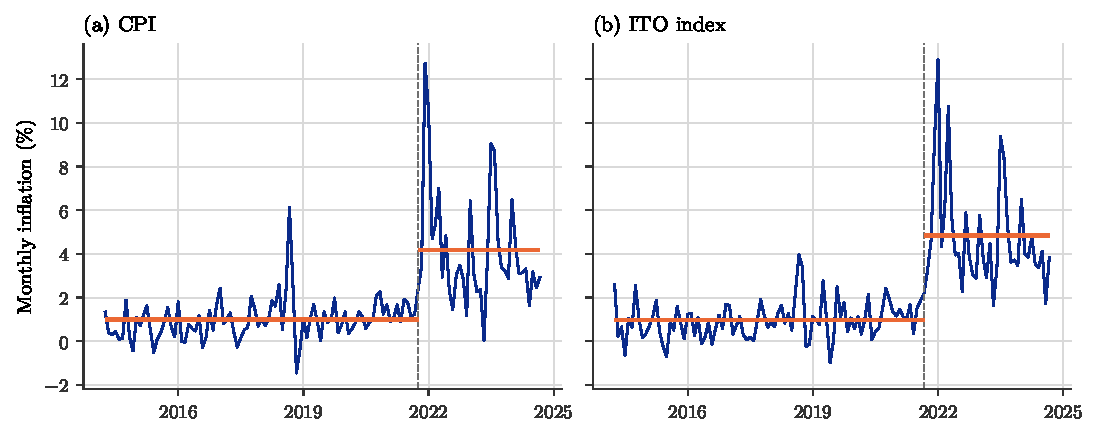
\includegraphics[width=0.92\linewidth]{../figures/fig3_breaks.pdf}
\caption{Monthly inflation of (a) the CPI and (b) the ITO index, with the Zivot--Andrews break (dashed) and the mean inflation
before and after it.}\label{fig:breaks}
\end{figure}

\textbf{Finding.} For CPI inflation the statistic is $\ZaTufe$ against critical values of $\ZaCvOne$ (1\%) and $\ZaCvFive$ (5\%):
the unit root is rejected in favour of stationarity around a shift after \ZaTufeBreak, with $k = \ZaTufeLags$. At this break
$\hat\theta = \ZaTufeTheta$ percentage points with $t = \ZaTufeTtheta$, while the trend is small and not significant ($t = \ZaTufeTbeta$).
Mean monthly inflation is \ZaTufeBefore\% before the break and \ZaTufeAfter\% after. The ITO index gives the same picture
($\ZaIto$, break after \ZaItoBreak; $t = \ZaItoTtheta$ for the shift and $\ZaItoTbeta$ for the trend; mean inflation \ZaItoBefore\%
and \ZaItoAfter\%). For the USD loan rate in levels the unit root is not rejected even when a break is allowed ($\ZaUsdL$); its
difference is stationary ($\ZaUsdD$). For real card spending growth, with the \ZaRealLags{} lags chosen by AIC, the statistic is
$\ZaReal$ and does not reject.

\textbf{Interpretation.} Monthly inflation in this sample is better described as stationary with one shift in its level in autumn
2021 than as $I(1)$; the trend allowed by Model A is not significant in either index. Two independently compiled price indices agree on the timing within a month. The log price levels are then
$I(1)$ with a break in their drift, not $I(2)$. The $I(2)$ result of version 1 for \texttt{tufe} is explained by testing the level of an
exponentially growing series and by ignoring this shift.

\section{Conclusions and limitations}

\begin{itemize}
  \item USD loan rate: $I(1)$, robust to every model, lag criterion and break; the same as in version 1.
  \item Consumer prices (CPI and ITO index): in logs, $I(1)$ with one shift in mean inflation in autumn 2021. Without the break the
  ADF test with AIC cannot exclude $I(2)$; version 1's $I(2)$ in levels is mainly a consequence of exponential growth.
  \item Card spending: the monthly data contain a calendar effect of about 25\% between four- and five-Friday months. In logs, per
  week and in real terms, the evidence points to $I(1)$ (BIC, KPSS); AIC selects 12 lags because of the annual pattern and then
  does not reject.
  \item Limitations: one break only, in the intercept (Model A), with the number of lags fixed across candidate dates; tests for two breaks, seasonal unit roots or ARIMA and VAR models, which the
  README of version 1 listed but did not carry out, are not included. 127 monthly observations give tests of limited power.
\end{itemize}

\section*{References}
{\small
Dickey, D. A., Fuller, W. A. (1979). Distribution of the estimators for autoregressive time series with a unit root.
\textit{Journal of the American Statistical Association}, 74(366), 427--431.\\
Dickey, D. A., Pantula, S. G. (1987). Determining the order of differencing in autoregressive processes. \textit{Journal of
Business \& Economic Statistics}, 5(4), 455--461.\\
Kwiatkowski, D., Phillips, P. C. B., Schmidt, P., Shin, Y. (1992). Testing the null hypothesis of stationarity against the
alternative of a unit root. \textit{Journal of Econometrics}, 54(1--3), 159--178.\\
MacKinnon, J. G. (1994). Approximate asymptotic distribution functions for unit-root and cointegration tests. \textit{Journal
of Business \& Economic Statistics}, 12(2), 167--176.\\
MacKinnon, J. G. (2010). Critical values for cointegration tests. Queen's Economics Department Working Paper No.~1227, Queen's
University.\\
Said, S. E., Dickey, D. A. (1984). Testing for unit roots in autoregressive-moving average models of unknown order.
\textit{Biometrika}, 71(3), 599--607.\\
Zivot, E., Andrews, D. W. K. (1992). Further evidence on the great crash, the oil-price shock, and the unit-root hypothesis.
\textit{Journal of Business \& Economic Statistics}, 10(3), 251--270.\\
statsmodels documentation: \texttt{adfuller}, \texttt{kpss}, \texttt{zivot\_andrews}.

\smallskip
An AI coding assistant was used in writing the code and in preparing this note. All numbers are generated from
\texttt{figures/*.csv} by \texttt{make\_paper.py}.
}

\end{document}
